\begin{table*}[t]\centering\small
\caption{Exploratory test errors in mph. Neural values are mean $\pm$ sample standard deviation across three seeds; references are frozen single runs.}
\begin{tabular}{lrrrrrr}\toprule
Method & MAE15 & MAE30 & MAE60 & RMSE15 & RMSE30 & RMSE60\\\midrule
Persistence & 3.482 & 4.173 & 5.321 & 6.374 & 7.983 & 10.250\\
Historical average & 4.187 & 4.187 & 4.187 & 7.852 & 7.852 & 7.852\\
Random Forest & 2.972 & 3.423 & 3.896 & 5.438 & 6.374 & 7.255\\
XGBoost & 2.920 & 3.376 & 3.874 & 5.777 & 6.911 & 7.993\\
Temporal GRU & 3.119 $\pm$ 0.001 & 3.811 $\pm$ 0.001 & 4.929 $\pm$ 0.002 & 6.112 $\pm$ 0.006 & 7.674 $\pm$ 0.004 & 9.721 $\pm$ 0.005\\
GRU + GAT & 3.099 $\pm$ 0.001 & 3.780 $\pm$ 0.002 & 4.881 $\pm$ 0.003 & 6.067 $\pm$ 0.004 & 7.606 $\pm$ 0.006 & 9.619 $\pm$ 0.003\\
\bottomrule\end{tabular}
\end{table*}

The common scored target counts at 15/30/60 minutes are 1,246,273/1,246,258/1,246,222. Overlapping forecasts are dependent; these counts are not independent trials.


Among the main comparison rows, the lowest 60-minute MAE is XGBoost (3.874 mph); the lowest 60-minute RMSE is Random Forest (7.255 mph). These are descriptive rankings, not test-based model-selection decisions. MAE measures average error size; RMSE puts greater emphasis on large misses.


\begin{table}[t]\centering\small
\caption{Learning-rate search: pooled headline tuning-validation MAE, mph, seed42. An asterisk marks the selected candidate in each family.}
\begin{tabular}{lrr}\toprule
Family & Rate & MAE\\\midrule
Temporal GRU* & 0.001 & 3.3346\\
Temporal GRU & 0.0003 & 3.3412\\
GRU + GAT* & 0.001 & 3.3057\\
GRU + GAT & 0.0003 & 3.3203\\
\bottomrule\end{tabular}
\end{table}

\begin{table}[t]\centering\small
\caption{Exploratory test MAPE, percent. Neural values average seeds; low positive speeds can inflate this metric.}
\begin{tabular}{lrrr}\toprule
Method & 15min & 30min & 60min\\\midrule
Persistence & 8.57 & 10.77 & 14.39\\
Historical average & 13.03 & 13.03 & 13.03\\
Random Forest & 8.07 & 9.81 & 11.71\\
XGBoost & 8.04 & 10.06 & 12.59\\
Temporal GRU & 8.28 & 10.69 & 14.68\\
GRU + GAT & 8.25 & 10.62 & 14.55\\
\bottomrule\end{tabular}
\end{table}

\begin{table}[t]\centering\small
\caption{Controlled seed42 ablations: test MAE, mph. Auxiliary controls have one seed; neighbour control also has multi-seed evidence.}
\begin{tabular}{lrrr}\toprule
Variant & 15min & 30min & 60min\\\midrule
GRU + GAT & 3.098 & 3.778 & 4.877\\
Self-loop graph & 3.109 & 3.802 & 4.923\\
Uniform neighbours & 3.101 & 3.785 & 4.891\\
No dropout & 3.075 & 3.756 & 4.847\\
\bottomrule\end{tabular}
\end{table}

\begin{table*}[t]\centering\small
\caption{Neighbour-access control: test MAE mean $\pm$ sample standard deviation, mph, over seeds42/43/44. Small seed spread is not a significance test.}
\begin{tabular}{lrrr}\toprule
Variant & 15min & 30min & 60min\\\midrule
GRU + GAT & 3.099 $\pm$ 0.001 & 3.780 $\pm$ 0.002 & 4.881 $\pm$ 0.003\\
Self-loop graph & 3.116 $\pm$ 0.006 & 3.809 $\pm$ 0.007 & 4.931 $\pm$ 0.007\\
\bottomrule\end{tabular}
\end{table*}

\begin{table}[t]\centering\small
\caption{Hybrid and its exact frozen constituent forecasts: test MAE, mph. This graph row is seed42, not a three-seed average.}
\begin{tabular}{lrrr}\toprule
Method & 15min & 30min & 60min\\\midrule
XGBoost & 2.920 & 3.376 & 3.874\\
Graph seed42 & 3.098 & 3.778 & 4.877\\
Selected blend & 2.920 & 3.376 & 3.874\\
\bottomrule\end{tabular}
\end{table}

Across seeds, graph MAE at 60 minutes is 4.881 mph, lower than self-loop control (4.931 mph). This is a measured comparison, not proof of causal congestion propagation or statistical significance.


The temporal baseline has mean 60-minute MAE 4.929 mph; frozen XGBoost has 3.874 mph. Graph-model change versus XGBoost is -26.00\% reduction (a negative value means worse error). Architecture, representation and training protocols differ from trees, so this comparison alone does not attribute differences to neighbour information.


Reserved-validation selection chose XGBoost weight $\lambda=1$. A pure endpoint won, so selection did not establish blend value. Test blend MAE at 15/30/60 minutes is 2.920/3.376/3.874 mph.


\begin{table*}[t]\centering\small
\caption{60-minute test MAE by target period, mph. Neural scores are seed means.}
\begin{tabular}{lrrrr}\toprule
Method & Peak & Off-peak & Weekday & Weekend\\\midrule
Random Forest & 5.954 & 3.379 & 4.041 & 3.333\\
XGBoost & 6.308 & 3.261 & 4.073 & 3.098\\
Temporal GRU & 7.751 & 4.220 & 5.308 & 3.454\\
GRU + GAT & 7.691 & 4.174 & 5.251 & 3.435\\
\bottomrule\end{tabular}
\end{table*}

\begin{table*}[t]\centering\small
\caption{Recorded fitting cost. Minutes are mean wall time per fit, including validation; contention, pauses and overlapping fits prevent isolated speed comparisons. Counts include inactive attention-score parameters in self/uniform modes.}
\begin{tabular}{lrrrr}\toprule
Variant & Parameters & Seeds & Epoch range & Minutes/fit\\\midrule
Temporal GRU & 3912 & 3 & 35--50 & 16.5\\
GRU + GAT & 5384 & 3 & 35--48 & 23.5\\
Self-loop graph & 5384 & 3 & 30--48 & 23.8\\
Uniform neighbours & 5384 & 1 & 48--48 & 27.8\\
No dropout & 5384 & 1 & 50--50 & 24.7\\
\bottomrule\end{tabular}
\end{table*}

No negative outputs occurred in any of the eleven neural fits (17,015,400 raw test forecasts per fit, including unscored targets). Outputs were not clipped. The unconstrained head does not guarantee physical bounds on other inputs.


In the seed42 sensor-level comparison, graph MAE is lower than self-only for 168 of 207 sensors and higher for 39. The signed map retains both directions. These unweighted sensor comparisons differ from pooled valid-point MAE. The fixed sensor/day forecast and fixed attention example illustrate local behaviour, not universal improvement or causal road influence.


\begin{figure*}[t]\centering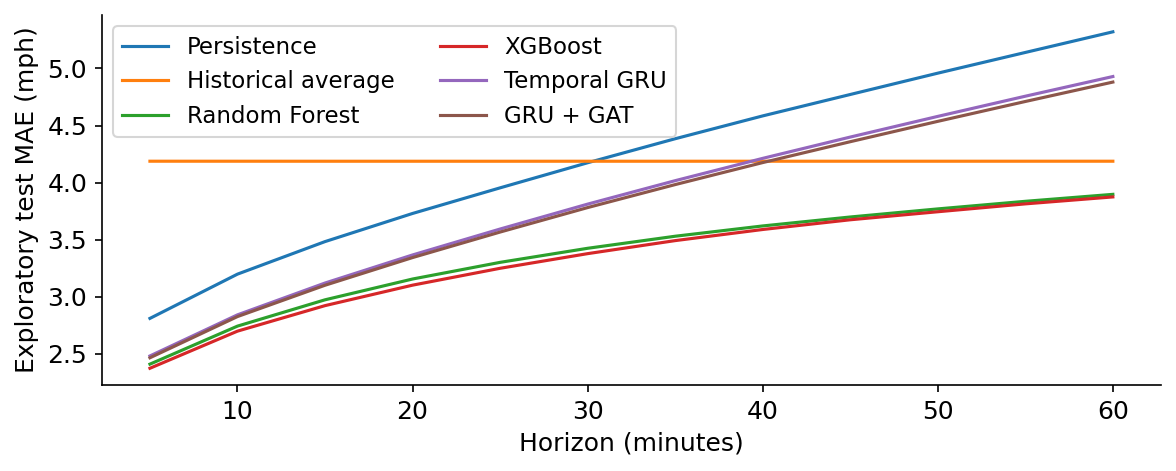
\includegraphics[width=.9\textwidth]{images/horizons.png}\caption{Exploratory test horizon errors; neural curves average seeds.}\end{figure*}

\begin{figure*}[t]\centering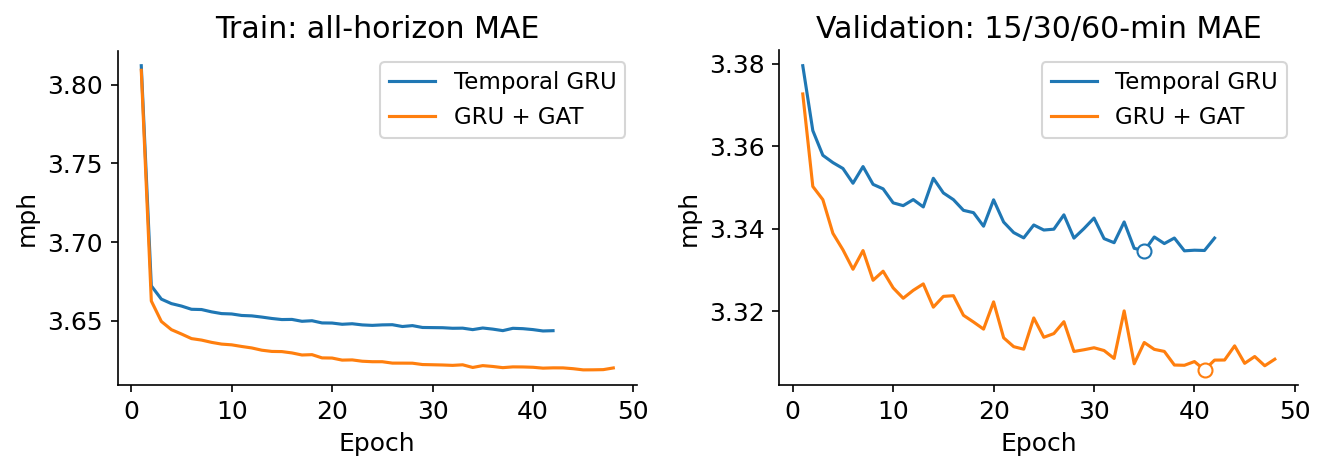
\includegraphics[width=.9\textwidth]{images/learning.png}\caption{Circles mark selected validation epochs. Different horizon aggregations and training/evaluation modes prevent interpreting vertical differences as a matched generalization gap.}\end{figure*}

\begin{figure*}[t]\centering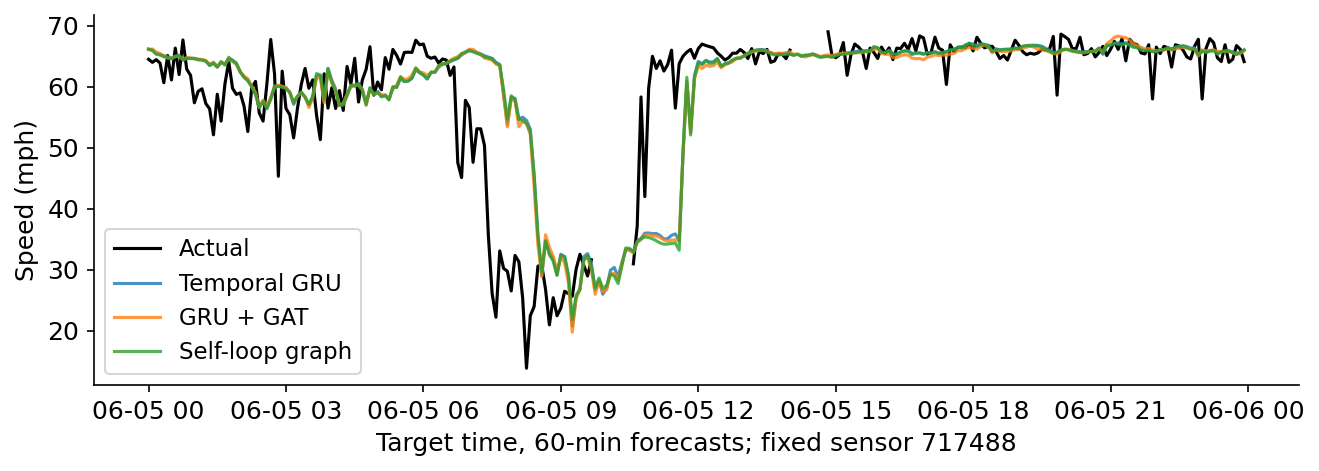
\includegraphics[width=.9\textwidth]{images/forecast.png}\caption{Fixed sensor/day example, not a network-wide performance claim.}\end{figure*}

\begin{figure*}[t]\centering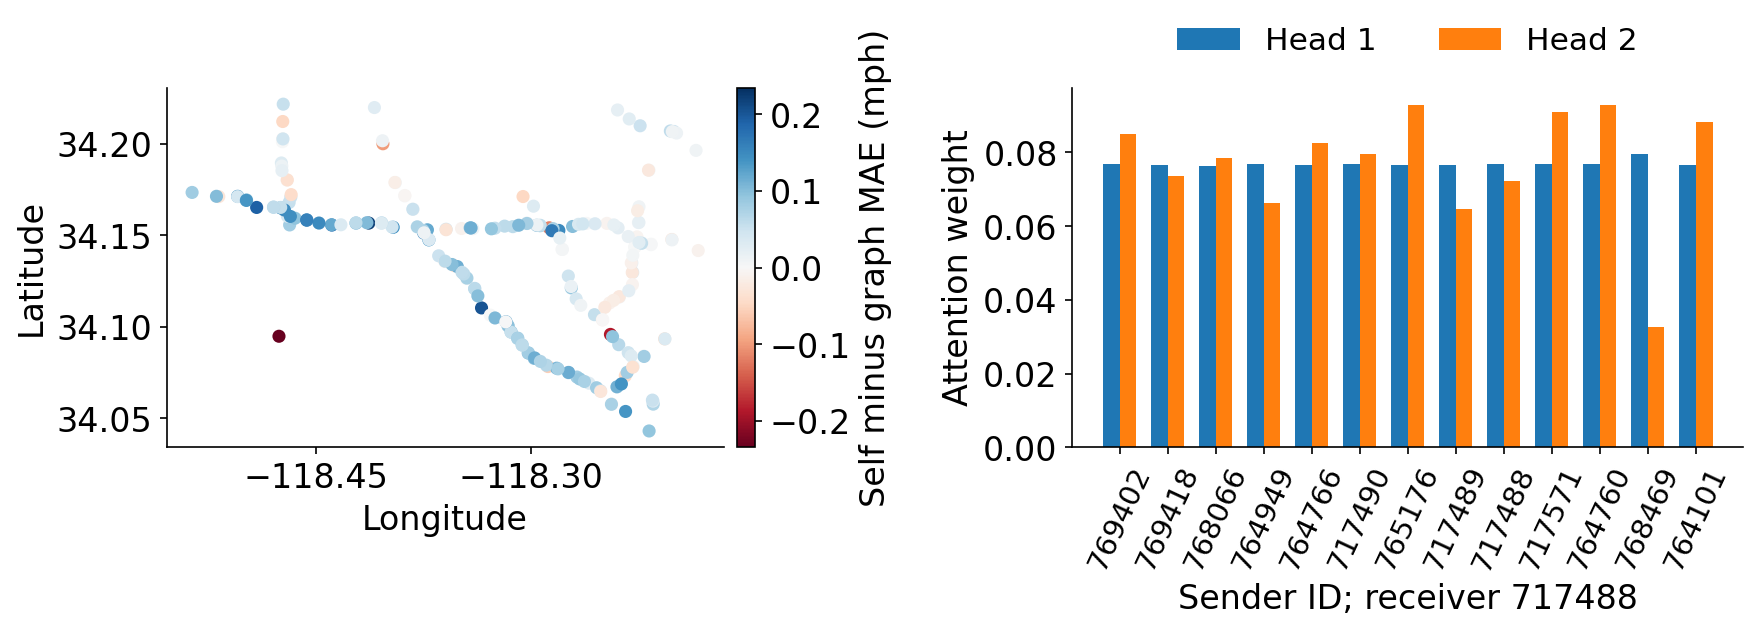
\includegraphics[width=.98\textwidth]{images/spatial_attention.png}\caption{Left: signed seed42 graph improvement, retaining regressions. Right: attention before dropout for a fixed receiver at the first test origin. Weights describe fitted behaviour, not physical causality.}\end{figure*}
